\documentclass{article}


\usepackage{siunitx} % Provides the \SI{}{} and \si{} command for typesetting SI units
\usepackage{graphicx} % Required for the inclusion of images
\usepackage{natbib} % Required to change bibliography style to APA
\usepackage{amsmath} % Required for some math elements 
\usepackage{listings}
\usepackage{placeins}
\usepackage{color}
\usepackage{caption}
\setlength\parindent{0pt} % Removes all indentation from paragraphs

\lstset{frame=tb,
  language=Matlab,
  aboveskip=3mm,
  belowskip=3mm,
  showstringspaces=false,
  columns=flexible,
  basicstyle={\small\ttfamily},
  numbers=none,
  numberstyle=\tiny\color{gray},
  keywordstyle=\color{blue},
  commentstyle=\color{green},
  stringstyle=\color{red},
  breaklines=true,
  breakatwhitespace=true,
  tabsize=3}
%\renewcommand{\labelenumi}{\alph{enumi}.} % Make numbering in the enumerate environment by letter rather than number (e.g. section 6)


\title{Lab 4 \\ Analysis of a Clipped Signals} % Title

\author{Aneesh Malhotra \\ G00844135} % Author name

\date{\today} % Date for the report

\begin{document}

\maketitle % Insert the title, author and date


% If you wish to include an abstract, uncomment the lines below
% \begin{abstract}
% Abstract text
% \end{abstract}

%----------------------------------------------------------------------------------------
%	SECTION 1
%----------------------------------------------------------------------------------------

\section{Introduction}



% If you have more than one objective, uncomment the below:
\begin{description}
\item[Objective] \hfill \\
The objective of this lab was to analyze the frequency response of an LTI system. Additionally we analyzed the spectrum of signals before and after they are clipped, that is leveled off at a particular threshold. 
\end{description}

\subsection{Frequency Response of LTI Systems}
The frequency response of an LTI system is the multiplier when the input to the system is an eigenfunction, namely a function of the form $e^{j \omega t}$. For a linear differential equation with constant coefficients, we see that the frequency response is given by $$\frac{a_n s^n + a_{n-1} s^n-1 + ... + a_0}{b_n s^n + b_{n-1} s^n-1 + ... + b_0}$$ where the $a_n$ coefficients are the coefficients of the $n$th derivative terms of the input and the $b_n$ coefficients are the coefficients of the $nth$ derivative of the output.
\subsection{Clipped Signals}
Clipped signals are signals that are leveled off beyond a particular threshold. For example, we can take a sinusoid and set all values whose absolute value is above the threshold to a constant, creating a square waveform. These changes can affect the spectrum of the signal. 

%----------------------------------------------------------------------------------------
%	SECTION 2
%----------------------------------------------------------------------------------------

\section{Main Body}

\subsection{Frequency Response}

We began by finding the poles and zeros of a particular differential equation given by $$y'' + 0.4y' + y = 0.2x'' + 0.3x' + x.$$
The frequency response of this system, analytically, is given by $$H(s) = \frac{0.2s^2 + 0.3s + 1}{s^2 + 0.4s + 1}.$$ Using Matlab's root function we found the zeros to be
 $$-0.75 \pm 2.106 i$$ and the poles to be $$-0.2 \pm 0.979 i.$$ The pole-zero plot is shown below:
 
\begin{figure}[!htbp]
\begin{minipage}{\linewidth}
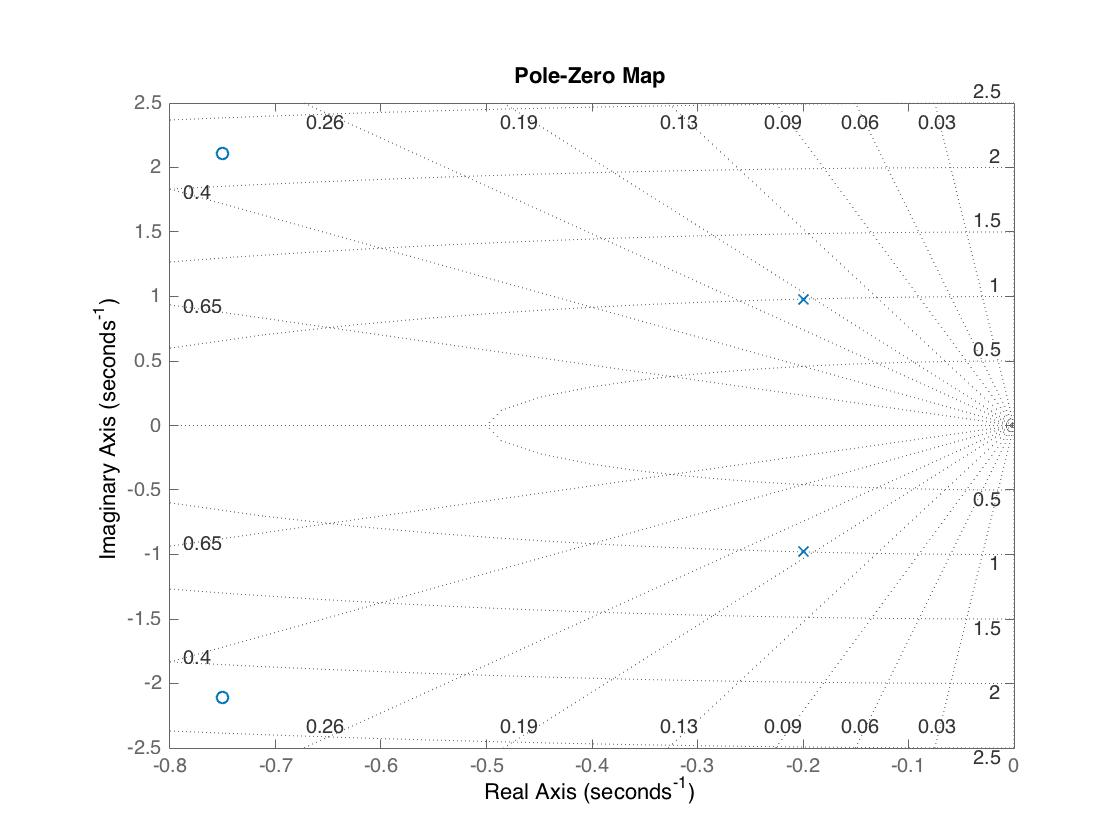
\includegraphics[width = 1\linewidth, height = 0.4\textheight]{polemap.jpg}
\captionof{figure}{Poles and zeros of the system on real-imaginary axis}
\end{minipage}
\end{figure}
\FloatBarrier
\subsection{Frequency Response of LTI Systems}
We found the frequency response of the system in the last equation using two methods: using the freqs command in Matlab, and by plotting it numerically. We obtained two plots:
\begin{figure}[!htbp]
\begin{minipage}{\linewidth}
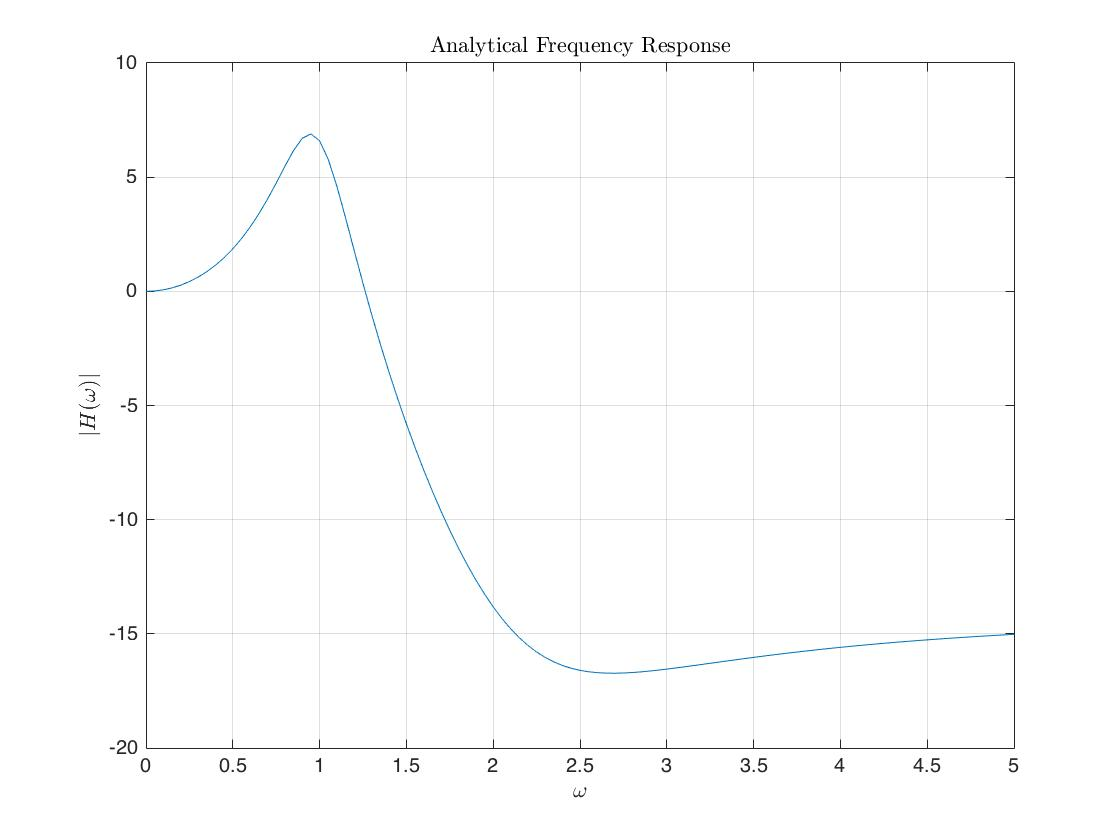
\includegraphics[width = 1\linewidth, height = 0.4\textheight]{analytical_freq.jpg}
\end{minipage}
\begin{minipage}{\linewidth}
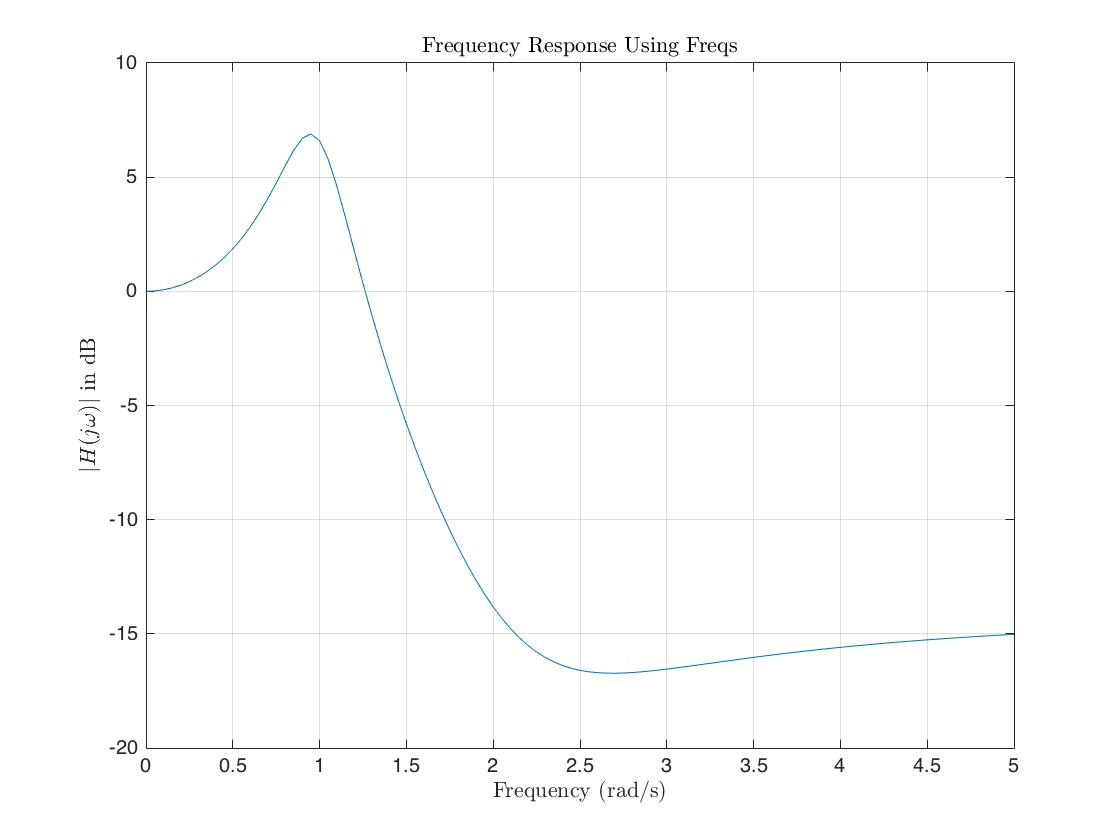
\includegraphics[width = 1\linewidth, height = 0.4\textheight]{num_freq.jpg}
\end{minipage}
\captionof{figure}{Analytical and numerical frequency responses look identical}
\end{figure}
We see that these figures are identical.
\FloatBarrier

We then analyzed a system whose frequency response is given by $$ H(s) = \frac{s^2 + \omega_0 ^2}{s^2 + 2\omega_0 \cos(\theta)s + \omega_0 ^2}.$$ Given $s = j\omega$, the frequency response will behave differently for different values of $\omega_0$ and $\theta$. For the case of $\theta  = \pi/3$, we see that if we let $s = j \omega$, frequencies at $\omega_0$ are attenuated, as shown in the plot below. 
\begin{figure}[!htbp]
\begin{minipage}{\linewidth}
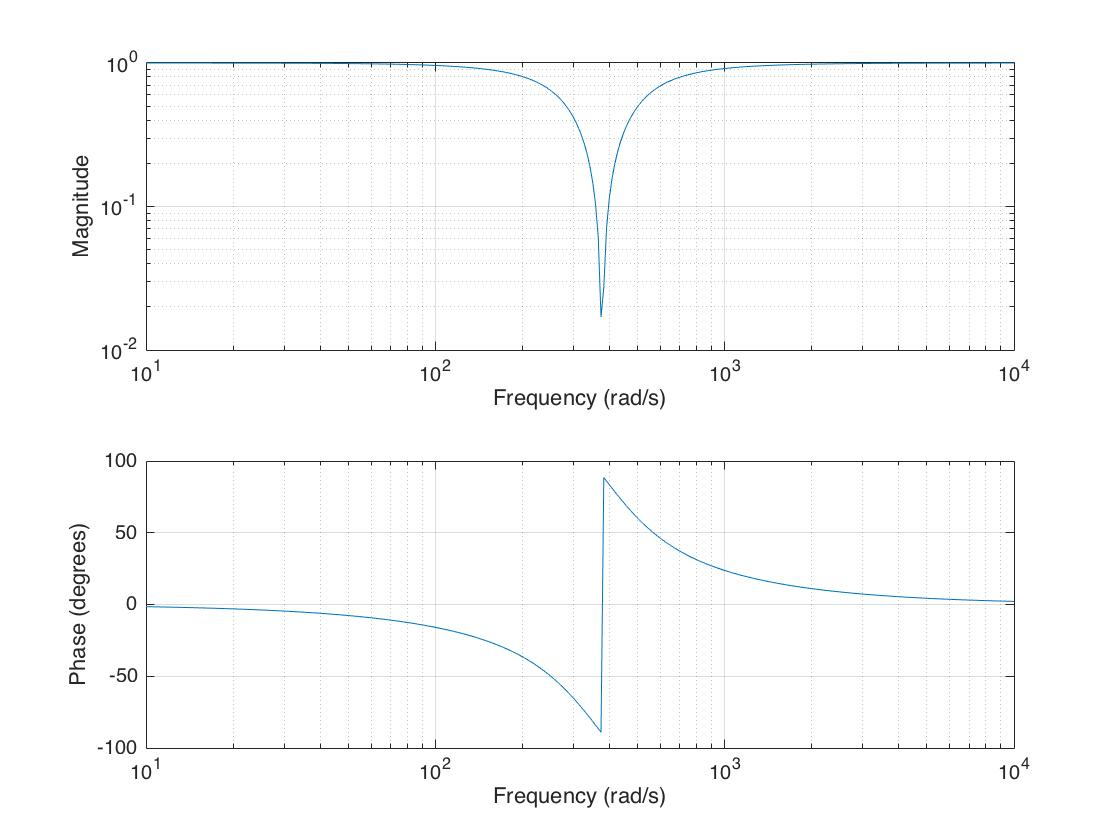
\includegraphics[width = 1\linewidth, height = 0.5\textheight]{freq_reponse1.jpg}
\captionof{figure}{Phase and magnitude of the frequency response when $\theta = \pi/3$}
\end{minipage}
\end{figure}
\FloatBarrier
We then set $\theta = \pi /2$. Since $\cos(\pi /2) = 0$, we see that the numerator and denominator of the frequency response are the same. Therefore, we see that the frequency response is always 1, as shown below.
\begin{figure}[!htbp]
\begin{minipage}{\linewidth}
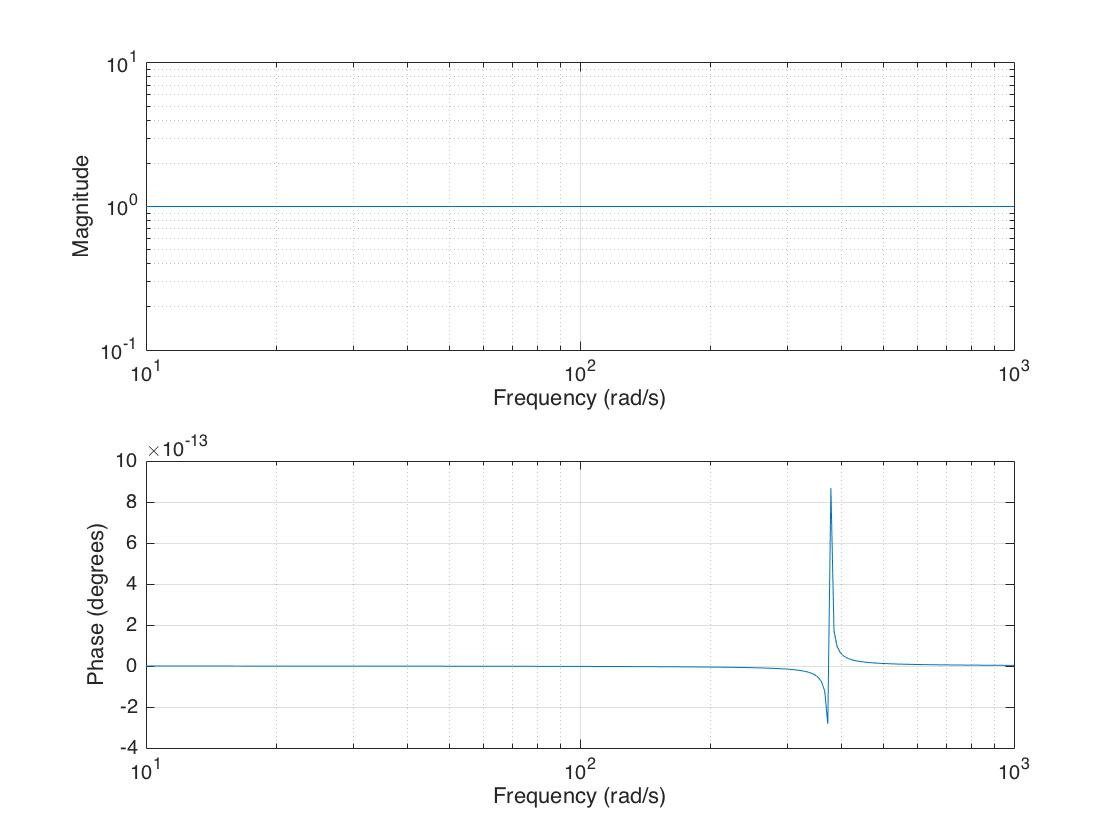
\includegraphics[width = 1\linewidth, height = 0.5\textheight]{freq_response2.jpg}
\captionof{figure}{When $\theta = \pi/2$, there is no attenuation}
\end{minipage}
\end{figure}
\FloatBarrier
\subsection{Amplitude Limiting Effects in LTI Systems}
Often in analyzing LTI systems, we want to prevent our input from reaching above a particular value. This can be achieved by "clipping" the signal above particular frequencies. We began by looking at a sinusoid with frequency $f_0 = 440$ with a sample rate of $f_s = 44,100$, with a total of $2^{16}$ samples. Using this information, we see that the duration of the signal should be roughly $1.486\si{s}$. We then clipped the signal such that its absolute value does not exceed $0.8$.
\begin{figure}[!htbp]
\begin{minipage}{\linewidth}
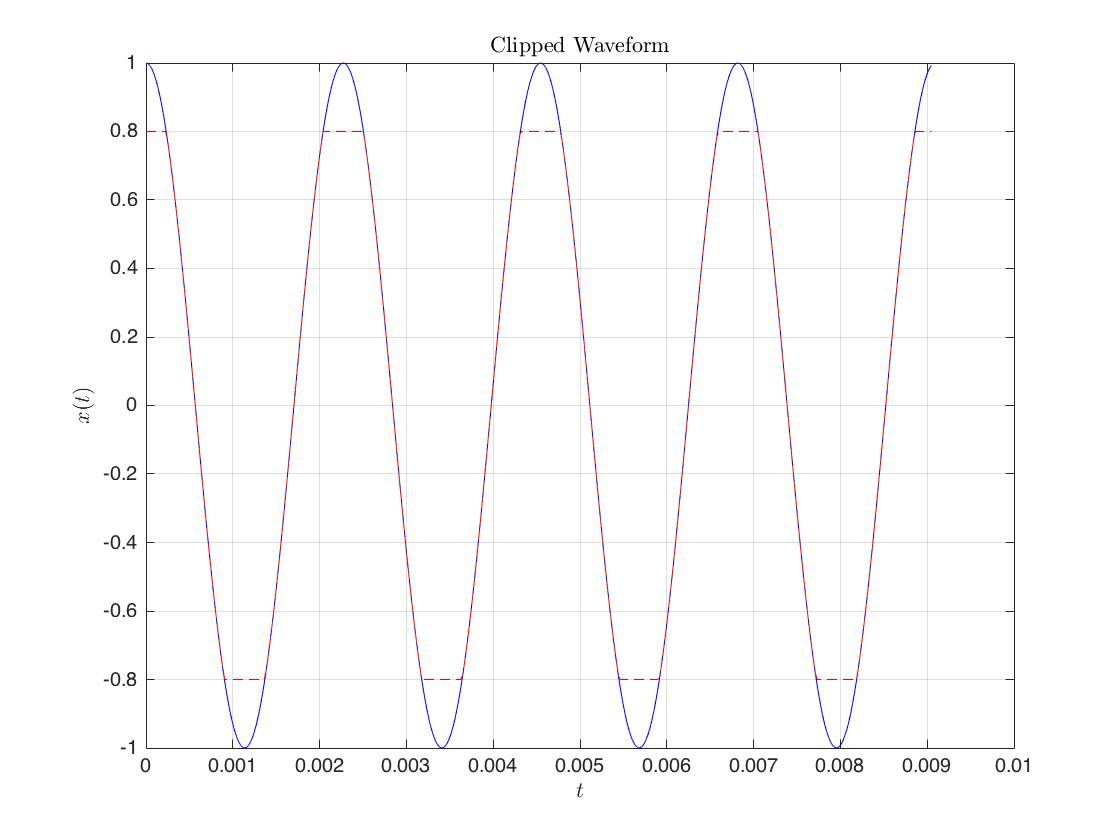
\includegraphics[width = 1\linewidth, height = 0.5\textheight]{clip1.jpg}
\captionof{figure}{Clipped Sinusoidal Waveform}
\end{minipage}
\end{figure}
\FloatBarrier
In this case, we see that we get a square wave. Noting that a cosine wave contains only two terms in its Fourier series, and a square contains infinitely many, we can analyze the spectrum to see that the clipped waveform has more harmonics than the original. This caused it to sound more like a trumpet rather than a tone, while it still maintained its pitch. Additionally, I noticed that clips of the waveform below $0.5$ were completely indistinguishable from each other. The plot of the spectrum is shown below. 
\begin{figure}[!htbp]
\begin{minipage}{\linewidth}
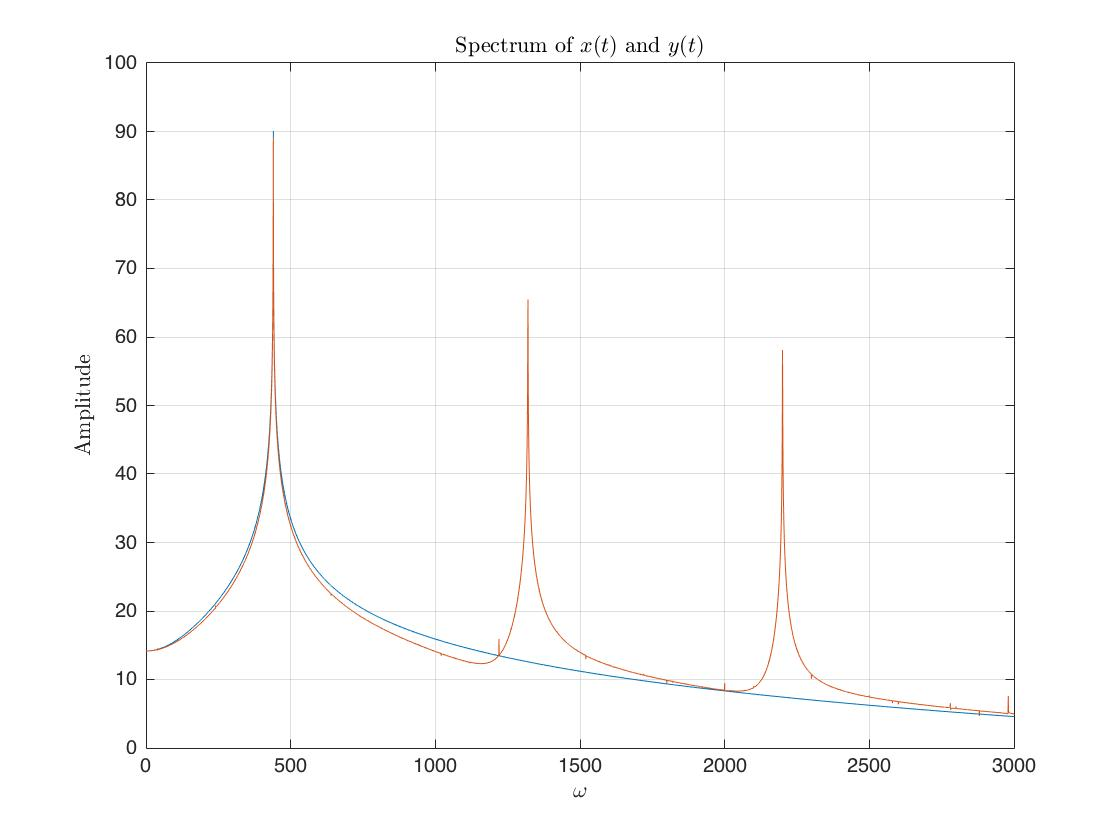
\includegraphics[width = 1\linewidth, height = 0.5\textheight]{trumpet.jpg}
\captionof{figure}{Spectrum of the sinusoid (blue) with the clipped sinusoid (orange)}
\end{minipage}
\end{figure}

\FloatBarrier
\subsection{Trumpet Signal}
We repeated the steps of the previous section for a trumpet signal. The trumpet signal, however, did not sound very different between clippings. The plot of the spectrum of both signals is shown below. 
\begin{figure}[!htbp]
\begin{minipage}{\linewidth}
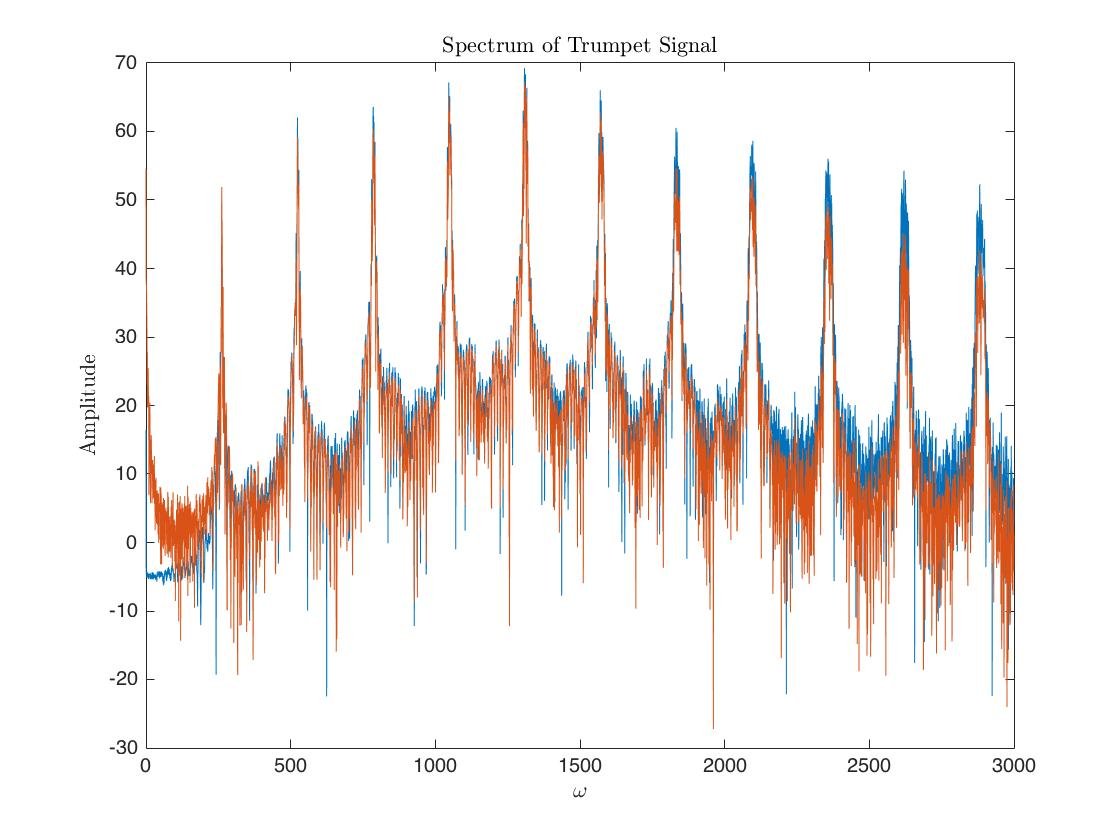
\includegraphics[width = 1\linewidth, height = 0.5\textheight]{trumpet1.jpg}
\captionof{figure}{Spectrum of a trumpet signal and a trumpet signal clipped for 0.5}
\end{minipage}
\end{figure}
We see that even though we truncated most of the signal in the time domain, we obtain similar results in the frequency domain. This may be because the trumpet signal is very complex and already has many harmonics, so the clipped waveform does not make a difference. When playing the sound I noticed no difference for various clipping thresholds.

\FloatBarrier
\subsection{Music Signal}
Finally, we repeated this process for a music signal. Like in the trumpet case, the signal likely was very complex and had many harmonics. Therefore, clipping did not have an effect qualitatively on the sound. We see that harmonically in the graph below, the original and clipped signals appear the same.

\begin{figure}[!htbp]
\begin{minipage}{\linewidth}
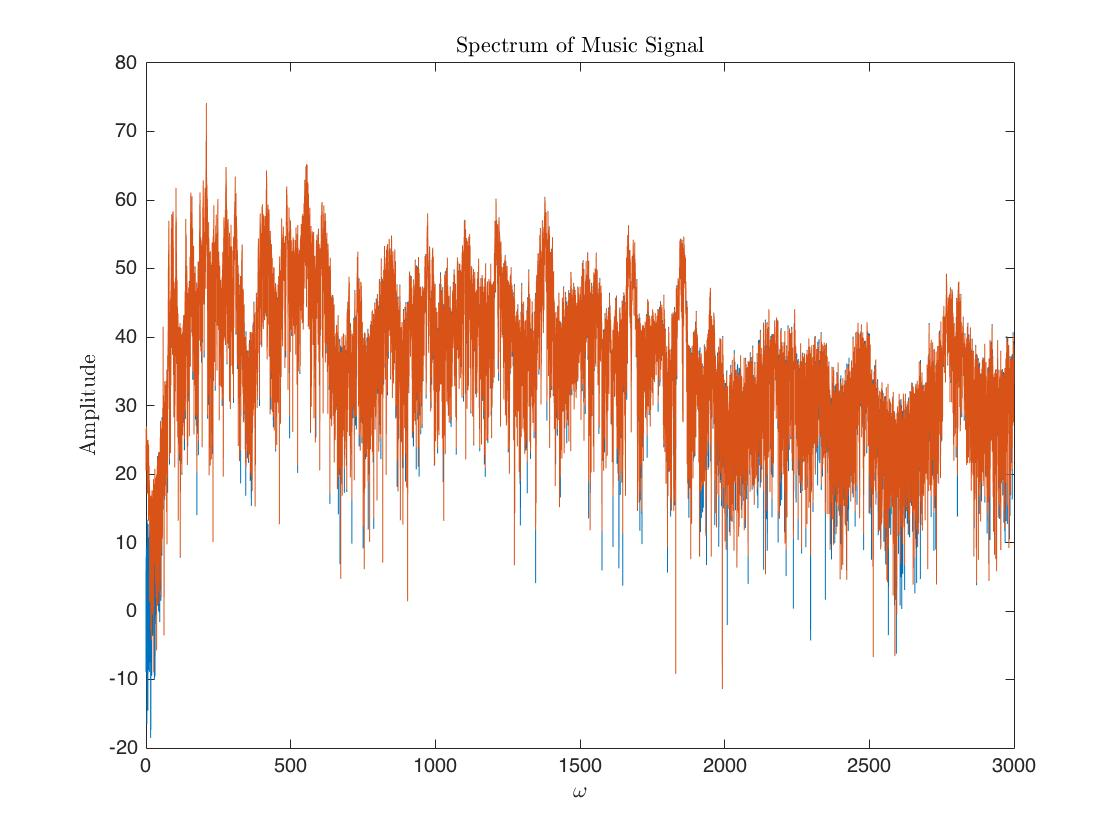
\includegraphics[width = 1\linewidth, height = 0.5\textheight]{music.jpg}
\captionof{figure}{Spectrum of a music signal (blue) and a clipped music signal (orange)}
\end{minipage}
\end{figure}

\FloatBarrier
\section{Conclusion}
In this lab we explored the poles and zeros of the frequency response, as well as the spectrum of clipped signals. Initially we looked at the frequency response of LTI systems. The frequency response indicates the strength of the output given the frequency of the input. We plotted the frequency response of a system in two ways: using Matlab's built in command and using our analytical solution. We saw that the plots were the same, once the units of the output was put in decibels. We then looked at a notch filter. This filter attenuated frequencies at a particular $\omega _0$ value, depending on the value of the $\theta$. If theta is an odd multiple of $\pi /2$, we saw that no attenuation occurs and the frequency response is always 1. Finally, we looked at clipped signals. Upon clipping a signals, we noticed that we form a square wave. Since square waves are formed by infinitely many harmonically related sine waves, we saw that there are infinitely many spikes in spectrum of the clipped signal. The clipped signal has more trumpet characteristic as well. I noticed that for heavily clipped signals, the sound of the signal becomes more noisy and becomes less clear. This was the case for both the trumpet and music signals. For clipping thresholds of 0.5 and 0.7, however, there was no noticeable difference.

\subsection{Appendix}
\subsection{Prelab Code}
\lstinputlisting{04_Aneesh_Malhotra_Matlab1.m}
\subsection{Lab Code}
\lstinputlisting{04_Aneesh_Malhotra_Matlab2.m}
%----------------------------------------------------------------------------------------
%	BIBLIOGRAPHY
%----------------------------------------------------------------------------------------
\section{References}

Lathi, B. P. Linear Systems and Signals. New York: Oxford UP, 2005. Print.

\end{document}